
%% bare_conf.tex
%% V1.4b
%% 2015/08/26
%% by Michael Shell
%% See:
%% http://www.michaelshell.org/
%% for current contact information.
%%
%% This is a skeleton file demonstrating the use of IEEEtran.cls
%% (requires IEEEtran.cls version 1.8b or later) with an IEEE
%% conference paper.
%%
%% Support sites:
%% http://www.michaelshell.org/tex/ieeetran/
%% http://www.ctan.org/pkg/ieeetran
%% and
%% http://www.ieee.org/

%%*************************************************************************
%% Legal Notice:
%% This code is offered as-is without any warranty either expressed or
%% implied; without even the implied warranty of MERCHANTABILITY or
%% FITNESS FOR A PARTICULAR PURPOSE! 
%% User assumes all risk.
%% In no event shall the IEEE or any contributor to this code be liable for
%% any damages or losses, including, but not limited to, incidental,
%% consequential, or any other damages, resulting from the use or misuse
%% of any information contained here.
%%
%% All comments are the opinions of their respective authors and are not
%% necessarily endorsed by the IEEE.
%%
%% This work is distributed under the LaTeX Project Public License (LPPL)
%% ( http://www.latex-project.org/ ) version 1.3, and may be freely used,
%% distributed and modified. A copy of the LPPL, version 1.3, is included
%% in the base LaTeX documentation of all distributions of LaTeX released
%% 2003/12/01 or later.
%% Retain all contribution notices and credits.
%% ** Modified files should be clearly indicated as such, including  **
%% ** renaming them and changing author support contact information. **
%%*************************************************************************


% *** Authors should verify (and, if needed, correct) their LaTeX system  ***
% *** with the testflow diagnostic prior to trusting their LaTeX platform ***
% *** with production work. The IEEE's font choices and paper sizes can   ***
% *** trigger bugs that do not appear when using other class files.       ***                          ***
% The testflow support page is at:
% http://www.michaelshell.org/tex/testflow/



\documentclass[conference]{IEEEtran}
\usepackage{mathrsfs}
\usepackage{amsmath}
\usepackage{amsthm}
\usepackage{amssymb}
\usepackage{amsfonts}
\usepackage{graphicx}
\usepackage{subfigure}
\usepackage{bm}
\usepackage{diagbox} 
\usepackage[colorlinks,linkcolor=blue]{hyperref}
\newtheorem{remark}{Remark}
% Some Computer Society conferences also require the compsoc mode option,
% but others use the standard conference format.
%
% If IEEEtran.cls has not been installed into the LaTeX system files,
% manually specify the path to it like:
% \documentclass[conference]{../sty/IEEEtran}





% Some very useful LaTeX packages include:
% (uncomment the ones you want to load)


% *** MISC UTILITY PACKAGES ***
%
%\usepackage{ifpdf}
% Heiko Oberdiek's ifpdf.sty is very useful if you need conditional
% compilation based on whether the output is pdf or dvi.
% usage:
% \ifpdf
%   % pdf code
% \else
%   % dvi code
% \fi
% The latest version of ifpdf.sty can be obtained from:
% http://www.ctan.org/pkg/ifpdf
% Also, note that IEEEtran.cls V1.7 and later provides a builtin
% \ifCLASSINFOpdf conditional that works the same way.
% When switching from latex to pdflatex and vice-versa, the compiler may
% have to be run twice to clear warning/error messages.






% *** CITATION PACKAGES ***
%
%\usepackage{cite}
% cite.sty was written by Donald Arseneau
% V1.6 and later of IEEEtran pre-defines the format of the cite.sty package
% \cite{} output to follow that of the IEEE. Loading the cite package will
% result in citation numbers being automatically sorted and properly
% "compressed/ranged". e.g., [1], [9], [2], [7], [5], [6] without using
% cite.sty will become [1], [2], [5]--[7], [9] using cite.sty. cite.sty's
% \cite will automatically add leading space, if needed. Use cite.sty's
% noadjust option (cite.sty V3.8 and later) if you want to turn this off
% such as if a citation ever needs to be enclosed in parenthesis.
% cite.sty is already installed on most LaTeX systems. Be sure and use
% version 5.0 (2009-03-20) and later if using hyperref.sty.
% The latest version can be obtained at:
% http://www.ctan.org/pkg/cite
% The documentation is contained in the cite.sty file itself.






% *** GRAPHICS RELATED PACKAGES ***
%
\ifCLASSINFOpdf
  % \usepackage[pdftex]{graphicx}
  % declare the path(s) where your graphic files are
  % \graphicspath{{../pdf/}{../jpeg/}}
  % and their extensions so you won't have to specify these with
  % every instance of \includegraphics
  % \DeclareGraphicsExtensions{.pdf,.jpeg,.png}
\else
  % or other class option (dvipsone, dvipdf, if not using dvips). graphicx
  % will default to the driver specified in the system graphics.cfg if no
  % driver is specified.
  % \usepackage[dvips]{graphicx}
  % declare the path(s) where your graphic files are
  % \graphicspath{{../eps/}}
  % and their extensions so you won't have to specify these with
  % every instance of \includegraphics
  % \DeclareGraphicsExtensions{.eps}
\fi
% graphicx was written by David Carlisle and Sebastian Rahtz. It is
% required if you want graphics, photos, etc. graphicx.sty is already
% installed on most LaTeX systems. The latest version and documentation
% can be obtained at: 
% http://www.ctan.org/pkg/graphicx
% Another good source of documentation is "Using Imported Graphics in
% LaTeX2e" by Keith Reckdahl which can be found at:
% http://www.ctan.org/pkg/epslatex
%
% latex, and pdflatex in dvi mode, support graphics in encapsulated
% postscript (.eps) format. pdflatex in pdf mode supports graphics
% in .pdf, .jpeg, .png and .mps (metapost) formats. Users should ensure
% that all non-photo figures use a vector format (.eps, .pdf, .mps) and
% not a bitmapped formats (.jpeg, .png). The IEEE frowns on bitmapped formats
% which can result in "jaggedy"/blurry rendering of lines and letters as
% well as large increases in file sizes.
%
% You can find documentation about the pdfTeX application at:
% http://www.tug.org/applications/pdftex





% *** MATH PACKAGES ***
%
%\usepackage{amsmath}
% A popular package from the American Mathematical Society that provides
% many useful and powerful commands for dealing with mathematics.
%
% Note that the amsmath package sets \interdisplaylinepenalty to 10000
% thus preventing page breaks from occurring within multiline equations. Use:
%\interdisplaylinepenalty=2500
% after loading amsmath to restore such page breaks as IEEEtran.cls normally
% does. amsmath.sty is already installed on most LaTeX systems. The latest
% version and documentation can be obtained at:
% http://www.ctan.org/pkg/amsmath





% *** SPECIALIZED LIST PACKAGES ***
%
%\usepackage{algorithmic}
% algorithmic.sty was written by Peter Williams and Rogerio Brito.
% This package provides an algorithmic environment fo describing algorithms.
% You can use the algorithmic environment in-text or within a figure
% environment to provide for a floating algorithm. Do NOT use the algorithm
% floating environment provided by algorithm.sty (by the same authors) or
% algorithm2e.sty (by Christophe Fiorio) as the IEEE does not use dedicated
% algorithm float types and packages that provide these will not provide
% correct IEEE style captions. The latest version and documentation of
% algorithmic.sty can be obtained at:
% http://www.ctan.org/pkg/algorithms
% Also of interest may be the (relatively newer and more customizable)
% algorithmicx.sty package by Szasz Janos:
% http://www.ctan.org/pkg/algorithmicx




% *** ALIGNMENT PACKAGES ***
%
%\usepackage{array}
% Frank Mittelbach's and David Carlisle's array.sty patches and improves
% the standard LaTeX2e array and tabular environments to provide better
% appearance and additional user controls. As the default LaTeX2e table
% generation code is lacking to the point of almost being broken with
% respect to the quality of the end results, all users are strongly
% advised to use an enhanced (at the very least that provided by array.sty)
% set of table tools. array.sty is already installed on most systems. The
% latest version and documentation can be obtained at:
% http://www.ctan.org/pkg/array


% IEEEtran contains the IEEEeqnarray family of commands that can be used to
% generate multiline equations as well as matrices, tables, etc., of high
% quality.




% *** SUBFIGURE PACKAGES ***
%\ifCLASSOPTIONcompsoc
%  \usepackage[caption=false,font=normalsize,labelfont=sf,textfont=sf]{subfig}
%\else
%  \usepackage[caption=false,font=footnotesize]{subfig}
%\fi
% subfig.sty, written by Steven Douglas Cochran, is the modern replacement
% for subfigure.sty, the latter of which is no longer maintained and is
% incompatible with some LaTeX packages including fixltx2e. However,
% subfig.sty requires and automatically loads Axel Sommerfeldt's caption.sty
% which will override IEEEtran.cls' handling of captions and this will result
% in non-IEEE style figure/table captions. To prevent this problem, be sure
% and invoke subfig.sty's "caption=false" package option (available since
% subfig.sty version 1.3, 2005/06/28) as this is will preserve IEEEtran.cls
% handling of captions.
% Note that the Computer Society format requires a larger sans serif font
% than the serif footnote size font used in traditional IEEE formatting
% and thus the need to invoke different subfig.sty package options depending
% on whether compsoc mode has been enabled.
%
% The latest version and documentation of subfig.sty can be obtained at:
% http://www.ctan.org/pkg/subfig




% *** FLOAT PACKAGES ***
%
%\usepackage{fixltx2e}
% fixltx2e, the successor to the earlier fix2col.sty, was written by
% Frank Mittelbach and David Carlisle. This package corrects a few problems
% in the LaTeX2e kernel, the most notable of which is that in current
% LaTeX2e releases, the ordering of single and double column floats is not
% guaranteed to be preserved. Thus, an unpatched LaTeX2e can allow a
% single column figure to be placed prior to an earlier double column
% figure.
% Be aware that LaTeX2e kernels dated 2015 and later have fixltx2e.sty's
% corrections already built into the system in which case a warning will
% be issued if an attempt is made to load fixltx2e.sty as it is no longer
% needed.
% The latest version and documentation can be found at:
% http://www.ctan.org/pkg/fixltx2e


%\usepackage{stfloats}
% stfloats.sty was written by Sigitas Tolusis. This package gives LaTeX2e
% the ability to do double column floats at the bottom of the page as well
% as the top. (e.g., "\begin{figure*}[!b]" is not normally possible in
% LaTeX2e). It also provides a command:
%\fnbelowfloat
% to enable the placement of footnotes below bottom floats (the standard
% LaTeX2e kernel puts them above bottom floats). This is an invasive package
% which rewrites many portions of the LaTeX2e float routines. It may not work
% with other packages that modify the LaTeX2e float routines. The latest
% version and documentation can be obtained at:
% http://www.ctan.org/pkg/stfloats
% Do not use the stfloats baselinefloat ability as the IEEE does not allow
% \baselineskip to stretch. Authors submitting work to the IEEE should note
% that the IEEE rarely uses double column equations and that authors should try
% to avoid such use. Do not be tempted to use the cuted.sty or midfloat.sty
% packages (also by Sigitas Tolusis) as the IEEE does not format its papers in
% such ways.
% Do not attempt to use stfloats with fixltx2e as they are incompatible.
% Instead, use Morten Hogholm'a dblfloatfix which combines the features
% of both fixltx2e and stfloats:
%
% \usepackage{dblfloatfix}
% The latest version can be found at:
% http://www.ctan.org/pkg/dblfloatfix




% *** PDF, URL AND HYPERLINK PACKAGES ***
%
%\usepackage{url}
% url.sty was written by Donald Arseneau. It provides better support for
% handling and breaking URLs. url.sty is already installed on most LaTeX
% systems. The latest version and documentation can be obtained at:
% http://www.ctan.org/pkg/url
% Basically, \url{my_url_here}.




% *** Do not adjust lengths that control margins, column widths, etc. ***
% *** Do not use packages that alter fonts (such as pslatex).         ***
% There should be no need to do such things with IEEEtran.cls V1.6 and later.
% (Unless specifically asked to do so by the journal or conference you plan
% to submit to, of course. )


% correct bad hyphenation here
\hyphenation{op-tical net-works semi-conduc-tor}


\begin{document}
%
% paper title
% Titles are generally capitalized except for words such as a, an, and, as,
% at, but, by, for, in, nor, of, on, or, the, to and up, which are usually
% not capitalized unless they are the first or last word of the title.
% Linebreaks \\ can be used within to get better formatting as desired.
% Do not put math or special symbols in the title.
\title{Asychronous Control for Markov Jump Lure's Systems}


% author names and affiliations
% use a multiple column layout for up to three different
% affiliations
%\author{\IEEEauthorblockN{Michael Shell}
%\IEEEauthorblockA{School of Electrical and\\Computer Engineering\\
%Georgia Institute of Technology\\
%Atlanta, Georgia 30332--0250\\
%Email: http://www.michaelshell.org/contact.html}
%\and
%\IEEEauthorblockN{Homer Simpson}
%\IEEEauthorblockA{Twentieth Century Fox\\
%Springfield, USA\\
%Email: homer@thesimpsons.com}
%\and
%\IEEEauthorblockN{James Kirk\\ and Montgomery Scott}
%\IEEEauthorblockA{Starfleet Academy\\
%San Francisco, California 96678--2391\\
%Telephone: (800) 555--1212\\
%Fax: (888) 555--1212}}

% conference papers do not typically use \thanks and this command
% is locked out in conference mode. If really needed, such as for
% the acknowledgment of grants, issue a \IEEEoverridecommandlockouts
% after \documentclass

% for over three affiliations, or if they all won't fit within the width
% of the page, use this alternative format:
% 
%\author{\IEEEauthorblockN{Michael Shell\IEEEauthorrefmark{1},
%Homer Simpson\IEEEauthorrefmark{2},
%James Kirk\IEEEauthorrefmark{3}, 
%Montgomery Scott\IEEEauthorrefmark{3} and
%Eldon Tyrell\IEEEauthorrefmark{4}}
%\IEEEauthorblockA{\IEEEauthorrefmark{1}School of Electrical and Computer Engineering\\
%Georgia Institute of Technology,
%Atlanta, Georgia 30332--0250\\ Email: see http://www.michaelshell.org/contact.html}
%\IEEEauthorblockA{\IEEEauthorrefmark{2}Twentieth Century Fox, Springfield, USA\\
%Email: homer@thesimpsons.com}
%\IEEEauthorblockA{\IEEEauthorrefmark{3}Starfleet Academy, San Francisco, California 96678-2391\\
%Telephone: (800) 555--1212, Fax: (888) 555--1212}
%\IEEEauthorblockA{\IEEEauthorrefmark{4}Tyrell Inc., 123 Replicant Street, Los Angeles, California 90210--4321}}




% use for special paper notices
%\IEEEspecialpapernotice{(Invited Paper)}




% make the title area
\maketitle

% As a general rule, do not put math, special symbols or citations
% in the abstract
\begin{abstract}
	This paper is concerned with the control problems for a class of discrete-time Lur'e systems with asynchronous controller. A hidden Markov model (HHM) is introduced to describe the asynchronous phenomenon between the systems mode and controller modes. The linear matrix inequality (LMI) approach is utilized to analyze the stability of the closed-loop system and $l_2$-gain performance.  Then a sufficient condition is proposed in the form of LMI to guarantee the stochastic stability of the closed-loop system, and to minimize the obtained $l_2$-gain from the disturbance to output, further more the asynchronous controller which contains a linear state feedback and a cone-bounded nonlinear output feedback can be designed by solving the given conditions. A simulation example is given to demonstrate the effectiveness of the proposed method. 
\end{abstract}

% no keywords




% For peer review papers, you can put extra information on the cover
% page as needed:
% \ifCLASSOPTIONpeerreview
% \begin{center} \bfseries EDICS Category: 3-BBND \end{center}
% \fi
%
% For peerreview papers, this IEEEtran command inserts a page break and
% creates the second title. It will be ignored for other modes.
\IEEEpeerreviewmaketitle
  
   

\section{Introduction}
	As an important class of stochastic switching systems, Markov jump systems (MJSs) have received considerable attention because of its powerful ability in modeling systems with abrupt change in parameters or system structures, for instance,  environmental disturbances, actuator failures, and variations in subsystems interconnections. Over the past few decades, a large number of works for stability analysis and the controller/filter design have been published[1234]. For example,    
	
%	但是,现如今存在的大多数成果都默认控制器的模态是已知的,且与系统模态保持一致,但是在实际应用中,这种情况可能会因为种种原因很难获得保证。也就是说,异步的情况是更合理的。 到现在,已经有少量的成果被提出来来解决这种情况,主要可以分成两种情况,我们分别称之为独立性模型,和异步控制模型。独立控制模型认为控制器的模态由一个新的Markov chin链描述,但是控制器的模态是相对于系统模态独立的,但是这种情况显然没有充分利用系统的信息,因此异步控制器模型被随之被研究。异步控制器认为,控制器的模态是有一个隐马尔科夫链控制的,且于系统模态有关。 在文献【wu】 的文章中首次系统的提出了基于隐马尔科夫模型的异步控制/滤波方法,同时该方法包含了同步的情况。...,在文献[23]中,带有不确定TP的异步线性马尔科夫稳定性问题进行了讨论。
%	
	In most existing works, it was  implicitly assumed that the information of system modes can be fully accessible for the controller/filter all the time, so that controller/filter modes can run synchronously with system modes. Unfortunately, in practical applications, it is rather difficult to satisfy this ideal assumption because of some unexpected factors, for instance, time delays, data dropouts and quantization in network control systems. In order to overcome this strict limitation, two research approach on control/filtering of MJSs were proposed, namely, mode-independent and asynchronous methods. In mode-independent methods\cite{mode_independent_T}\cite{mode_independent_wuhuaining}, the controller modes is independent with plant modes, which means have no use of system information and may result in some conservatism. Therefore, asynchronous methods on control/filtering problems for MJSs gain more attention in recent years. For example,  a piecewise homogeneous Markov chain was utilized to design an asynchronous $l_2$-$l_\infty$ filter for discrete-time MJSs with randomly occurred sensor nonlinearities in \cite{l2_filter_wu}. After that, in \cite{passive_wu}, a new strategy based on HMM framework was adopted in passivity-based asynchronous control problems, which covers the synchronous situation. Very recently, many works on asynchronous control/filtering problem of MJSs have been published based on this powerful model. For instance, asynchronous filter design of discrete-time Markov Jump Systems was discussed in \cite{filter_shenying}\cite{filter_zhangmeng}, the same issue was discussed in continuous-time domain in \cite{continus_filter_dongshanling}, and asynchronous $l_2$-$l_{\infty}$ control problem for discrete-time Markovian jump linear systems with partly accessible controller mode information was addressed in \cite{unknown_asynchronous_control}. 
%	在实际控制系统中,分线性是普遍存在的,有一种被称作洛尔系统的一种特殊系统近年来得到了广泛的关注。该系统的一般形式为,其中代表线性部分,代表扇形游街部分。在文献???中分别提出了一种控制手段,在文献??利用正态李雅普诺夫方程中利用这样的控制手段分析了带有未知参数的离散马尔科夫跳变系统,之后,在文献中,利用一种新型的李雅普诺夫方程对该类系统进行了重新的研究,并得到了更加不保守的条件。但是值得注意的是,目前前述论文对洛尔系统控制器的设计于分析都是同步的,也就是说,异步洛尔跳变系统尚未进行讨论,这也就激发了我们对这类进行的分析。本文的贡献如下,首先,我们设计了一个类似于文献???中采用的控制形式,但是是一个异步状态,输出反馈,并分析了其稳定性问题。其次,针对上述系统的l2性能进行了分析
%	论文贡献:1. 异步控制应用到洛尔系统中去,2.控制器包含了一个线性状态反馈控制器及一个非线性的异步输出反馈控制器。 

	On the other hand, nonlinearity is another common phenomenon universally exists in the practical control systems. Among many different descriptions of non-linear system, a special one called Lur'e system\cite{khnlil}, which is consisted of a linear part and a cone-bounded nonlinearity, has received a lot of attentions in recent years[some references]. Many excellent works have been published on stability analysis and controller design problems for Lur'e system. For example, the issue of absolute stabilization for Lur'e system with a sector bounded nonlinearity under control saturations was discussed in \cite{state_output_control_EB} and \cite{state_output_control_EB_continues}, respectively, in discrete-time and continues-time domain. The flexibility was increased due to a mode-dependent controller which consisted of a linear state-feedback and a cone-bound nonlinear output feedback was introduced, and was also universally adopted in many later works. In \cite{song_control}, stability and $l_2$-gain problem was discussed for a class of discrete-time nonlinear MJSs with actuator saturation and incomplete knowledge of transition probabilities by construct a stochastic quadratic candidate Lyapunov function. Almost at the same time, a new class of Lyapunov functions including the cone-bounded nonlinearity, Lur'e type Lyapunov function, was proposed to the stability analysis for discrete-time Lur'e systems in \cite{gonzaga}. Then, the stochastic Lur's type Lyapunov function was applied to solve the stochastic stability problem for a class of discrete-time Markov jump Lur'e systems in \cite{costaolv_control_1} and \cite{costaolv_control}. However, as we can know, the issue of stability and stabilization for discrete-time Lur'e systems with asynchronous controller have not been investigated yet, which motivates us for the current work. 
	
	In this paper, the stochastic stabilization and $l_2$-gain minimization problems was discussed for a class of discrete-time Markov Jump Lur'e system with asynchronous controller. The contribution of this paper are: (1) Design a asynchronous controller which consists of a liner state feedback and a cone-bound nonlinear output feedback(similar with \cite{gonzaga}) based on a Hidden Markov model. (2) A sufficient theorem in the from LMI was given to make sure the system is stochastic stabilize and minimize the $l_2$-gain performance. The rest of this paper is organized as follows: In Section II, we introduce the system model and give some preliminaries related to this paper.  Section III analysis the stochastic stability for a class of discrete-time Markov Jump Lur'e system.  Section IV deals with the $l_2$-gain minimization problem and design the asynchronous controller. A numerical example was provided to illustrate the effectiveness of the given theorems in Section V. Finally, we summarize the works of this paper in Section VI. 
%	文章的组织结构如下:第一部分主要提供了一一些预备知识,第二部分对系统的稳定性问题进行了讨论,第三部分考虑了外部扰动,并对系统的l2性能进行了分析。第四部分给出了一个例子来描述提出方法的可行性。
	
	 
	
	



% An example of a floating figure using the graphicx package.
% Note that \label must occur AFTER (or within) \caption.
% For figures, \caption should occur after the \includegraphics.
% Note that IEEEtran v1.7 and later has special internal code that
% is designed to preserve the operation of \label within \caption
% even when the captionsoff option is in effect. However, because
% of issues like this, it may be the safest practice to put all your
% \label just after \caption rather than within \caption{}.
%
% Reminder: the "draftcls" or "draftclsnofoot", not "draft", class
% option should be used if it is desired that the figures are to be
% displayed while in draft mode.
%
%\begin{figure}[!t]
%\centering
%\includegraphics[width=2.5in]{myfigure}
% where an .eps filename suffix will be assumed under latex, 
% and a .pdf suffix will be assumed for pdflatex; or what has been declared
% via \DeclareGraphicsExtensions.
%\caption{Simulation results for the network.}
%\label{fig_sim}
%\end{figure}

% Note that the IEEE typically puts floats only at the top, even when this
% results in a large percentage of a column being occupied by floats.


% An example of a double column floating figure using two subfigures.
% (The subfig.sty package must be loaded for this to work.)
% The subfigure \label commands are set within each subfloat command,
% and the \label for the overall figure must come after \caption.
% \hfil is used as a separator to get equal spacing.
% Watch out that the combined width of all the subfigures on a 
% line do not exceed the text width or a line break will occur.
%
%\begin{figure*}[!t]
%\centering
%\subfloat[Case I]{\includegraphics[width=2.5in]{box}%
%\label{fig_first_case}}
%\hfil
%\subfloat[Case II]{\includegraphics[width=2.5in]{box}%
%\label{fig_second_case}}
%\caption{Simulation results for the network.}
%\label{fig_sim}
%\end{figure*}
%
% Note that often IEEE papers with subfigures do not employ subfigure
% captions (using the optional argument to \subfloat[]), but instead will
% reference/describe all of them (a), (b), etc., within the main caption.
% Be aware that for subfig.sty to generate the (a), (b), etc., subfigure
% labels, the optional argument to \subfloat must be present. If a
% subcaption is not desired, just leave its contents blank,
% e.g., \subfloat[].


% An example of a floating table. Note that, for IEEE style tables, the
% \caption command should come BEFORE the table and, given that table
% captions serve much like titles, are usually capitalized except for words
% such as a, an, and, as, at, but, by, for, in, nor, of, on, or, the, to
% and up, which are usually not capitalized unless they are the first or
% last word of the caption. Table text will default to \footnotesize as
% the IEEE normally uses this smaller font for tables.
% The \label must come after \caption as always.
%
%\begin{table}[!t]
%% increase table row spacing, adjust to taste
%\renewcommand{\arraystretch}{1.3}
% if using array.sty, it might be a good idea to tweak the value of
% \extrarowheight as needed to properly center the text within the cells
%\caption{An Example of a Table}
%\label{table_example}
%\centering
%% Some packages, such as MDW tools, offer better commands for making tables
%% than the plain LaTeX2e tabular which is used here.
%\begin{tabular}{|c||c|}
%\hline
%One & Two\\
%\hline
%Three & Four\\
%\hline
%\end{tabular}
%\end{table}


% Note that the IEEE does not put floats in the very first column
% - or typically anywhere on the first page for that matter. Also,
% in-text middle ("here") positioning is typically not used, but it
% is allowed and encouraged for Computer Society conferences (but
% not Computer Society journals). Most IEEE journals/conferences use
% top floats exclusively. 
% Note that, LaTeX2e, unlike IEEE journals/conferences, places
% footnotes above bottom floats. This can be corrected via the
% \fnbelowfloat command of the stfloats package.




\section{Preliminaries}
Consider a class of discrete-time MJLS on a probability space ($\varOmega,\mathcal{F},\mathcal{P}$):
\begin{equation}\label{syseq}
	\left\{
	\begin{array}{lr}
		\begin{split}
			x_{k+1}&=A_{r(k)}x_k+F_{r(k)}\varphi(y_k)+B_{r(k)}u_k\\
			&+E^x_{r(k)}w_k, \quad y_k=C_{r(k)}x_k,
		\end{split}
		\\
		\begin{split}
			z_k= & C^z_{r(k)}x_k+G^z_{r(k)}\varphi(y_k)+D^z_{r(k)}u_k\\
				&+E^z_{r(k)}w_k
		\end{split}
		
	\end{array}
	\right.
\end{equation}\\
%where$A_{r(k)}, F_{r(k)}, B_{r(k)}, E^x_{r(k)}, C^z_{r(k)}, G^z_{r(k)}, D^z_{r(k)}$ and $E^z_{r(k)}$ represent the time-varying system matrices, all of which are pre-known and real, $x_k \in \mathbb{R}^{n_x}, u_k \in \mathbb{R}^{n_u}, y_k\in \mathbb{R}^{n_y}, z_k\in \mathbb{R}^{n_z}$, and $w_k\in\mathbb{R}^{n_w}$ are respectively the state, the control input, the output related to the nonlinearity, the controlled output and the exogenous disturbance vector of system \eqref{syseq} at the instant k.  
where $x_k\in\mathbb{R}^{n_x}, u_k\in\mathbb{R}^{n_u}, y_k\in\mathbb{R}^{n_y}, z_k\in\mathbb{R}^{n_z}$, and $w_k\in\mathbb{R}^{n_w}$ represent the state, the control input, the output related to the nonlinearity, the controlled output and the exogenous disturbance vector respectively. $A_{r(k)}, F_{r(k)}, B_{r(k)}, E^x_{r(k)}, C^z_{r(k)}, G^z_{r(k)}, D^z_{r(k)}$ and $E^z_{r(k)}$ represent the time-varying system matrices, all of which are pre-known and real.  
%Where $x_k\in\mathbb{R}^{n_x}$ is the state vector, $u_k\in\mathbb{R}^{n_u}$ is the control input, $y_k\in\mathbb{R}^{n_y}$ is the system output, $z_k\in\mathbb{R}^{n_z}$ is the control output, nad $w_k\in\mathbb{R}^{n_w}$ is the exogenous disturbance in $l_2[0,\infty)$, at the instant $k$. The saturation function $\rm{sat}(\cdot)$ is defined as follows: for any $u\in\mathbb{R}^{n_u}, \mathrm{sat}(u)_{(\ell)}=\mathrm{sign}u_{(\ell)} \min(\rho_{(\ell)},|u_{(\ell)}|),\forall\ell=1,\dots,n_u\}$, where $\ell$ represent the $\ell$th element of the vector and  the vector $0<\rho<\mathbb{R}^n_u$ is assumed to be given. $\{r(k),k\geq0\}$ is a Markov chain taking values in a finite set $\mathcal{N}=\{1,2,\dots,N\}$ with mode TPs:
%The saturation function $\rm{sat}(\cdot)$ is defined as follows: for any $u\in\mathbb{R}^{n_u}, \mathrm{sat}(u)_{(\ell)}=\mathrm{sign}u_{(\ell)} \min(\rho_{(\ell)},|u_{(\ell)}|),\forall\ell=1,\dots,n_u\}$, where $\ell$ represent the $\ell$th element of the vector and  the vector $0<\rho<\mathbb{R}^n_u$ is assumed to be given. $\{r(k),k\geq0\}$ is a Markov chain taking values in a finite set $\mathcal{N}=\{1,2,\dots,N\}$ with mode TPs:
%The saturation function $\rm{sat}(\cdot)$ is defined as follows:
%\begin{equation}
%\mathrm{sat}(u)_{(\ell)}=\mathrm{sign}(u_{(\ell)}) \min(\rho_{(\ell)},|u_{(\ell)}|),
%\end{equation}
%where $\ell \in \{1,\cdots,m\}$ represent the $\ell$th element of the vector and  the pre-given vector $\rho>0$.
$\{r(k),k\geq0\}$ is a Markov chain taking values in a positive integer set $\mathcal{N}=\{1,2,\dots,N\}$ with mode TPs:
\begin{equation}
	\Pr\{r(k+1)=j|r(k)=i\}=\pi_{ij}
\end{equation}
Clearly, for all $i,j\in\mathcal{N}$, $\pi_{ij}\in[0,1]$, and $\sum_{j=1}^{N}\pi_{ij}=1$ for each mode $i$. The system matrices in \eqref{syseq} at instant $k$ can be expressed as $A_i,F_i,B_i,E^x_i,C^z_i,G^z_i,D^z_i$ and $E^z_i$, which are real known constant matrices with appropriate dimensions, and the related transition probability matrix is described as $\mathit{\Pi}=\{\pi_{ij}\}$.\\
\\
\textbf{Assumption 1:} The function $\varphi(\cdot): \mathbb{R}^{n_y}\rightarrow\mathbb{R}^{n_y}$ satisfies:\\ 
(1) $\varphi(0)=0$ and \\
(2) there exists a diagonal positive definite matrix $\varOmega \in\mathbb{R}^{n_y\times n_y}$ such that: 
\begin{equation}\label{cbs}
\varphi_{(\ell)}(y)[\varphi(y)-\varOmega y ]_{(\ell)}\leq 0.
\end{equation}
where for all $y\in\mathbb{R}^{n_y}$, $\ell \in\{1,\dots,n_y\}$. And in this case we say that the nonlinearity $\varphi(\cdot) $ satisfies it's own cone bounded sector conditions and to be decentralized. According to \eqref{cbs} we have:
\begin{equation}\label{scieq}
	SC(y,\varLambda):= \varphi^{\mathrm{'}}(y)\varLambda[\varphi(y)-\varOmega y]\leq0,
\end{equation}
%where $\varLambda$ is any diagonal postive semidefinite matrix, and $\varOmega$ is consider to be given. From the Assumption 1, we have that inequality \label{scieq} yields to $[\varOmega y]_{(\ell)}[\varphi(y)-\varOmega y]_{(\ell)}\leq0, \forall\ell=1,\dots,n_y, \forall y\in\mathbb{R}^{n_y}$, which implies: $\forall y \in \mathbb{R}^{n_y}, 0\leq\varphi^{\mathrm{T}}(y)\varLambda\varphi(y) \leq \varphi^{\mathrm{T}}(y)\varLambda\varphi(y) \leq y^{\mathrm{T}}\varOmega\varLambda\varOmega y$.
where $\varLambda$ is any diagonal positive semidefinite matrix, and $\varOmega$ is pre-given. From the Assumption 1, we get:
\begin{equation}
[\varOmega y]_{(\ell)}[\varphi(y)-\varOmega y]_{(\ell)}\leq0,
\end{equation}
which implies:
\begin{equation}
 0\leq\varphi^{\mathrm{'}}(y)\varLambda\varphi(y) \leq \varphi^{\mathrm{'}}(y)\varLambda\varOmega y \leq y^{\mathrm{'}}\varOmega\varLambda\varOmega y
\end{equation}\\
\textbf{Definition 1:} System \eqref{syseq} is said to be locally stochastically stable if for $w_(k)=0$ and any initial condition $x_0\in \mathcal{D}_0$, $r_0\in \mathcal{N}$, the following formulation holds:
\begin{equation}
	\|x\|^2_2=\sum_{k=0}^{\infty}\mathbb{E}[\|x_k\|^2]<\infty.
\end{equation} 
Where in this case the set $\mathcal{D}_0 \subset \mathbb{R}^{p}$ is said to be the domain of stochastic stability of the origin. \\
\\
Define $\mathcal{F}_k$ as the $\sigma$-field generated by the random variables $x_k$ and $r(k)$. We define next the class of exogenous disturbances with bounded energy and the finite $\ell_2$-induced              norm.
\\
\textbf{Definition 2}: For $\zeta>0$, set $\mathcal{W}_{\zeta} $ is defined as follows:
\begin{equation}
	\begin{split}
		\mathcal{W}_{\zeta}&:=\{w=\{w_k\}_{k\in\mathbb{N}};w_k\in\mathbb{R}^{m}, k\in\mathbb{N}, w_k \ \text{is} \\
		&\mathcal{F}_k\text{-measureable}, \text{and}\  \|w\|^2_2=\sum_{k=0}^{\infty}\mathbb{E}(\|w_k\|)^2<\zeta.\\
	\end{split}
\end{equation}
The finite $\ell_2$-induced gain associated with the closed-loop system \eqref{syseq} with $x_0=0$ between the disturbance $w=\{w_k\}_{k\in\mathbb{N}}$ and controlled output $z=\{z_k\}_{k\in\mathbb{N}}$ is equal or less than $\gamma$ if for every $w\in\mathcal{W}_{\zeta}$ then we have
\begin{equation}
\|z\|^2_2=\sum_{k=0}^{\infty}\mathbb{E}\left[\|z_k\|^2\right] \leq \gamma^{2}\|w\|^2_2=\gamma^{2}\sum_{k=0}^{\infty}\mathbb{E}\left[\|w_k\|^2\right].
\end{equation}
In this paper, we consider the following controller:
\begin{equation}\label{asycontroller}
u_k=K_{\sigma(k)}x_k+\varGamma_{\sigma(k)}\varphi(y_k) 
\end{equation}
where $K_{\sigma(k)}\in \mathbb{N}^{n_u\times n_x}$ is a time-varying controller gain matrix, and $\varGamma_{\sigma(k)}\in \mathbb{N}^{n_u\times n_y}$ is a time-varying nonlinear output feedback gain matrix. The parameter $\{\sigma(k),k\geq0\}$ takes values in another pre-given positive integer set, which is marked as $\mathcal{M}=\{1,2,\dots,M\}$ subject to the pre-known conditional probability matrix $\varPhi=\{\mu_{im} \}$, the probabilities of which are defined by
\begin{equation}
\Pr\{\sigma(k)=\phi|r(k)=i\}=\mu_{i\phi}.
\end{equation}
Where for all $i\in\mathcal{N}, \phi\in\mathcal{M}, \mu_{i\phi}\in [0,1]$, and $\sum_{\phi=1}^{M}\mu_{i\phi}=1$ for each $i\in\mathcal{N}$.
\begin{remark}
	Similar with \cite{passive_wu}, a HHM was introduced to describe the asynchronous phenomenon appears between the controller and the plant. Its easy to find that, the controller designed here consists a linear state feedback and a nonlinear output feedback which satisfy cone-bounded condition based on assumption 1. Different form the synchronous controller introduced in \cite{song_control} and \cite{costaolv_control_1}, the controller adopted in this paper is a asynchronous controller, which means the controller mode and the plant mode may different at the same time. Obviously, when the probability matrix $\varPhi$ is unit matrix, the controller mode will run synchronously with the plant, asynchronous controller becomes a synchronous controller, which means the asynchronous controller considered in this paper takes the synchronization as a special case. 
\end{remark} 
%\textbf{Remark 1}: In practice, the information of the system modes can not be fully accessed to controller or not fully accurate, that is, the actual modes of system are hidden to the controller, which leads to the controller don't synchronize with system modes. Thus, we introduce $\sigma(k)$ to present the relationship between system modes and controller modes, and the set $(r(k),\sigma(k),\varPi,\varPhi)$ constructs a hidden Markov model. \\
%\\
%In this paper, we define the dead-zone nonlinearity $\delta(u)$ as follows:$\delta(u)=u-\mathrm{sat}(u)$, for any $u\in\mathbb{R}^{m}$. 
Combing the asynchronous controller \eqref{asycontroller} and system \eqref{syseq} we have the following closed-loop system:
%\begin{equation}\label{close_system_equation}
%\left\{ 
%\begin{array}{lr}
%\begin{split}
%x_{k+1}=&(A_i+B_iK_m)x_k+(F_i+B_i\varGamma_m)\varphi(y_k)\\
%&+E_i^xw_k\\
%\end{split}
%\\
%\begin{split}
%z_k=&(C^z_i+D_i^zK_m)x_k+(G^z_i+D^z_i\varGamma_m)\varphi(y_k)\\
%&+E^z_iw_k
%\end{split}
%\end{array}
%\right.
%\end{equation} 
%\\
\begin{equation}\label{close_system_equation_2}
\left\{
\begin{array}{lr}
\begin{split}
x_{k+1}=\bar{A}_{i\theta}x_k+\bar{F}_{i\theta}\varphi_{i}(C_ix_k)+E_i^xw_k\\
\end{split}
\\
\begin{split}
z_k=\bar{C}^{z}_{i\theta}x_k+\bar{G}^{z}_{i\theta}\varphi_{i}(C_ix_k)+E^z_iw_k
\end{split}
\end{array}
\right.
\end{equation} 
Where, for $i \in \mathcal{N}, \phi \in \mathcal{M}$
\begin{equation} \notag
\begin{aligned}
\bar{A}_{i\phi}=A_{i}+B_{i}K_{\phi},  \qquad \bar{F}_{i\phi}=F_{i}+B_{i}\varGamma_{i\phi} \\
\bar{C}^{z}_{i\phi}=C^{z}_{i}+D^{z}_{i}K_{\phi}, \qquad \bar{G}^{z}_{i\phi}=G^{z}_{i}+D^{z}_{i}\varGamma_{\phi}
\end{aligned}
\end{equation}

%We consider a generalized local sector condition $\delta(u)=u-\mathrm{sat}(u)$, and use $\rho$ to denote the bounds of saturation function $\mathrm{sat}(u)$. For given matrices $H_m\in\mathbb{R}^{n+p}$, we define the set $\mathcal{S}(H_m,\rho):=\{\xi\in\mathbb{R}^{n_x+n_y};-\rho\leq H_m\xi\leq\rho, \forall m\in \mathcal{M} \}$.
%\\
%\textbf{Lemma 3}. Consider matrices $\widehat{K_m}=[K_m \ \varGamma_m]\in\mathbb{N}^{m\times(n+p)}$ and $\widehat{J_m}=[J_{1,m} \ J_{2,m}]\in\mathbb{N}^{m\times(n+p)}$. If $\widehat{x}=[x^{'} \ \varphi^{'}(C_ix) ]^{'} \in \mathcal{S}(\widehat{K_m}-\widehat{J_m},\rho)$, for $u=K_mx+\varGamma_m\varphi(C_ix)$ we have that the nonlinearity $\delta(u)$ satisfies the following sector condition for any diagonal positive definite matrix $T_m\in\mathbb{R}^{m\times m}$:
%\begin{equation}
%\begin{split}
%SC_u(i,m,u,x,T_m):= &\delta^{'}(u)T_m^{-1}[\delta(u)-\widehat{J_m}\widehat{x}]\leq 0.
%\end{split}
%\end{equation}
%\\




\section{Main Result}
 
%LavFunction:
%\begin{equation}
%	V(x_k,r(k)) = x_k^{'}P_{r(k)}x_k+2\varphi^{'}(C_{r(k)}x_k)\varDelta_{r(k)}\varOmega_{r(k)} C_{r(k)}x_k
%\end{equation}
%
%\begin{equation}
%	\begin{split}
%		E\{\varDelta V(k)\}=&E\{V(k+1,x_{k+1},r(k+1)=j|x_k,r(k)=i\}\\
%							&-V(k,x_k,i)
%	\end{split}
%\end{equation}
%
%
%\begin{equation}
%\begin{split}
%&E\{V(x_{k+1},r(k+1)=j|x_k,r(k)=i\}\\
%&=E\{x_{k+1}^{'}(\sum_{j=1}^{N}\pi_{ij}P_{j})x_{k+1} + 2\sum_{j=1}^{N}\pi_{ij}\varphi^{'}(C_jx_{k+1})\varDelta_{j}\varOmega_{j}C_jx_{k+1}  \}\\
%&=E\{x_{k+1}^{'}(\sum_{j=1}^{N}\pi_{ij}P_{j})x_{k+1} +x^{'}_{k+1}\sum_{j=1}^{N}\pi_{ij}C^{'}_{j}\varOmega_{j}\varDelta_{j}\varphi(C_jx_{k+1})    \}
%\end{split}
%\end{equation}
\subsection{stochastic stability analysis}
In this subsection, we focus on the stochastic stability analysis for the closed-loop system \eqref{close_system_equation_2}. A sufficient condition presented in the form of LMI was derived to guarantee the considered Lur'e system stochastically stable.

Theorem1. System \eqref{close_system_equation_2} with $x_0=0$ and $w_{k}=0$ is stochastically stable, if for all $i \in \mathcal{N}$ and $\phi \in \mathcal{M}$, there exist positive definite matrices $\bar{P_i} \in \mathbb{R}^{n_x\times n_x}$, $R_{i\phi } \in \mathbb{R}^{(n_x+n_y)\times(n_x+n_y)}$, matrices $K_{\phi} \in \mathbb{R}^{n_u\times n_x}$, $\varGamma_{\phi} \in \mathbb{R}^{n_u \times n_y}$ and positive semidefinite matrix $T_{i}\in \mathbb{R}^{n_y}$ to  ensure \eqref{condition_1_1} and \eqref{condition_1_2} hold.
\begin{equation}\label{condition_1_1}
\begin{bmatrix}
-R_{i\theta}&\mathscr{H}_{i\phi}\\
*&\mathscr{P}_{i}
\end{bmatrix}<0
\end{equation}


\begin{equation}\label{condition_1_2}
\begin{bmatrix}
\mathscr{S}_{i\phi}&\mathscr{N}_{i\phi}\\
*&\mathscr{L}_{i\phi}
\end{bmatrix}<0
\end{equation}


%\begin{equation}\notag
%\begin{bmatrix}
%-R_{i\theta}&\sqrt{\pi_{i1}}\hat{A}^{'}_{i\theta}&\cdots&\sqrt{\pi_{iN}}\hat{A}^{'}_{i\theta}\\ \\
%\sqrt{\pi_{i1}}\hat{A}_{i\theta}&-\bar{P_1}&0&0\\ \\
%\vdots &0&\ddots&0\\ \\
%\sqrt{\pi_{iN}}\hat{A}_{i\theta}&0&0& -\bar{P}_{N}
%\end{bmatrix}<0
%\end{equation}
%
%
%\begin{equation}\notag
%\begin{bmatrix}
%	\mathscr{S}_{i\phi}&
%	\sqrt{u_{i1}}\mathscr{N}_{i1}&
%	\cdots&
%	\sqrt{u_{iM}}\mathscr{N}_{iM}\\  \\
%	\sqrt{u_{i1}}\mathscr{N}_{i1}&
%	L_{i1}&0&0\\  \\
%	\vdots&0&\ddots&0\\  \\
%	\sqrt{u_{iM}}\mathscr{N}_{iM}&0&0&L_{iM}
%				 
%\end{bmatrix}<0
%\end{equation}
where \\
\begin{equation}\notag
	\begin{aligned}
	\mathscr{N}_{i\phi}&=\begin{bmatrix}
	\sqrt{u_{i1}}L_{i1}&\sqrt{u_{i2}}L_{i2}&\cdots&\sqrt{u_{iM}}L_{iM}
	\end{bmatrix}\\
	\mathscr{P}_{i\phi}&=\mathrm{diag} \{-\bar{P}_{1},-\bar{P}_{2},\dots,-\bar{P}_{N}  \}\\
	\mathscr{L}_{i\phi}&=\mathrm{diag} \{-L_{i1},-L_{i2},\dots,-L_{iM}  \}\\
		\mathscr{H}_{i\phi}&=\begin{bmatrix}
			\sqrt{\pi_{i1}}\hat{A}_{i\phi}\\
			\sqrt{\pi_{i2}}\hat{A}_{i\phi}\\
			\vdots\\
			\sqrt{\pi_{i_N}}\hat{A}_{i\phi}
		\end{bmatrix}^{'}, \quad
		\hat{A}_{i\theta}=\begin{bmatrix}
		\bar{A}_{i\theta}&\bar{F}_{i\theta}
		\end{bmatrix}  \\
		L_{i\phi}&=\begin{bmatrix}
		\bar{P}_{i}&0\\
		*&R_{i1}
		\end{bmatrix}, \quad
		L_{i\phi}=\begin{bmatrix}
		I_{n_x}&0\\
		*&R_{i1}
		\end{bmatrix}\\
		H_{i\theta}&=\begin{bmatrix}
			-I_{n_x}&C^{'}_{i}\varOmega_{i}T_{i} \\
			*&-2T_{i}
		\end{bmatrix}\\
		\mathscr{S}_{i\phi}&= \begin{bmatrix}
			-\bar{P}_{i}&0\\
			*&H_{i\phi}
		\end{bmatrix}\\
%		\mathscr{N}_{i\phi}&=\begin{bmatrix}
%				\sqrt{u_{i1}}\begin{bmatrix}
%				\bar{P}_{i}&0\\
%				*&R_{i1}
%			\end{bmatrix}&
%			\dots&	
%			\sqrt{u_{iM}}\begin{bmatrix}
%				\bar{P}_{i}&0\\
%				*&R_{iM}
%			\end{bmatrix}&
%		\end{bmatrix} \\
%		\mathscr{L}_{i\phi}&=\mathrm{diag}\Bigg\{\begin{bmatrix}
%			-I_{n_x}&0\\
%			*&-R_{i1}
%		\end{bmatrix},\dots,
%		\begin{bmatrix}
%			-I_{n_x}&0\\
%			*&-R_{iM}
%		\end{bmatrix}  \Bigg\} 
	\end{aligned}
\end{equation}

Proof: We first construct a Lyapunov function in the form of \eqref{lyapunov_funciton}.
\begin{equation}\label{lyapunov_funciton} 
	V(k,x_k,r(k))=x^{'}_{k}P_{r(k)}x_{k}
\end{equation}


And $P_{r(k)}=\bar{P}^{-1}_{r(k)}$. Let $\mathbb{E}\{\varDelta V(k)\}=\mathbb{E}\{V(k+1,x_{k+1},r(k+1)=j|x_k,r(k)=i \}-V(k,x_k,i)$ and it is easy to find that
\begin{equation} \label{lypfunction}
	\mathbb{E}\{\varDelta V(k)\}=\mathbb{E}\{x^{'}_{k+1}X_{i} x_{k+1} \}-V(k,x_k,i)
\end{equation} 
Where $X_{i} = \sum_{j=1}^{N}\pi_{ij}P_{j}$. Based on system \eqref{close_system_equation_2} we can further obtain \\
\begin{equation}
	\begin{split}
		\mathbb{E}\{x^{'}_{k+1}X_{i} x_{k+1} \}& = \sum_{\phi=1}^{M} u_{i\phi} \hat{x}^{'}_{k} \hat{A}^{'}_{i\phi}X_{i}\hat{A}_{i\phi}\hat{x}_{k}\\
		&=\hat{x}^{'}_{k} \Big( \sum_{\phi=1}^{M}u_{i\phi}\hat{A}^{'}_{i\phi}X_{i}\hat{A}_{i\phi}\Big) \hat{x}_{k} 
	\end{split}
\end{equation}
Where $\hat{x}_{k}=(x^{'}_k,\varphi^{'}_{i}(C_{i}x_{k}))^{'}$. Which implies
\begin{equation} \label{leq18}
	\begin{split}
		\mathbb{E}\{\varDelta V(k)\}=\hat{x}^{'}_{k} \Big( \sum_{\phi=1}^{M}u_{i\phi}\hat{A}^{'}_{i\phi}X_{i}\hat{A}_{i\phi}\Big) \hat{x}_{k} -x^{'}_{k}P_{i}x_{k}
	\end{split}
\end{equation}
Denoting $h_{i\phi} = \mathrm{diag}\{P_{i}, I_{n_x+n_y},\{\mathrm{diag}(I_{n_x},R^{-1}_{i\phi})^{M}_{\phi=1} \} \}$ and using $h_{i\phi}$ to pre- and post-multiplying the inequality given in \eqref{condition_1_2}, respectively, then we can get \\
\begin{equation}\label{st}
\begin{bmatrix} 
	\hat{\mathscr{S}}_{i\phi}&
\sqrt{u_{i1}}I&
\cdots&
\sqrt{u_{iM}}I\\
\sqrt{u_{i1}}I&L_{i1}&0&0\\ 
\vdots&0&\ddots&0\\
\sqrt{u_{iM}}I&0&0&
L_{iM}

\end{bmatrix} <0
\end{equation}
Where, for all $\phi\in\mathcal{M}$
\begin{equation} \notag
	\begin{aligned}
		\hat{\mathscr{S}}_{i\phi}=\begin{bmatrix}
			-P_{i }&0\\
			*&H_{i\phi}
		\end{bmatrix},
		L_{i\phi} = \begin{bmatrix}
			-I_{n_x}&0\\
			*&-R^{-1}_{i\phi}
		\end{bmatrix}
	\end{aligned}
\end{equation}
Applying Schur complement to the inequality above, we can further obtain \\
\begin{equation} \label{cons}
\sum_{\phi=1}^{M}u_{i\phi} \begin{bmatrix}
I&0\\
*&R_{i\phi}
\end{bmatrix} + \begin{bmatrix}
-P_{i }&0\\
*&H_{i\phi}
\end{bmatrix} <0
\end{equation}
\eqref{cons} multiply $(x^{'}_k,\hat{x}^{'}_{k})^{'}$ on left and it's transpose on the right. We get\\
\begin{equation} \label{iq11}
	\begin{split}
		&\hat{x}^{'}_{k}\sum_{\phi=1}^{M}u_{i\phi}R_{i\phi}\hat{x}+x^{'}_{k}(\sum_{\phi=1}^{M}u_{i\phi}I_{n_x})x_{k}-x^{'}_{k}I_{n_x}x_{k}\\
		&-x^{'}_{k}P_{i}x_{k}-2SC(i,x_k,T_i)<0
	\end{split}
\end{equation}
Noting that $\sum_{\phi=0}^{M}u_{i\phi}=1$, then $\sum_{\phi=0}^{M}u_{i\phi}I_{n_x}=I_{n_x}$, that implies the \eqref{iq11} is equivalent to:
\begin{equation} \label{iq1}
\hat{x}^{'}_{k}\sum_{\phi=1}^{M}u_{i\phi}R_{i\phi}\hat{x}_k-x^{'}_{k}P_{i}x_{k}-2SC(i,x_k,T_i)<0
\end{equation}
Applying Schur complement to inequality \eqref{condition_1_1}. We can obtain \\
\begin{equation} \label{iq2}
\hat{A}_{i\phi}X_{i}\hat{A}_{i\phi}<R_{i\phi}
\end{equation}
Combining inequalities \eqref{iq1} and \eqref{iq2}, it's easy to find that \\
\begin{equation} \label{leq22}
	\begin{split}
	\hat{x}^{'}_{k}\sum_{\phi=1}^{M} u_{i\phi}(\hat{A}_{i\phi}X_{i}&\hat{A}_{i\phi}) \hat{x}_{k} - x^{'}_{k}P_{i}x_{k}\\
	&-2SC(i,x_k,T_i)<0
	\end{split}
\end{equation}
Consider the condition given in \eqref{leq18}, it is easy to obtain that
\begin{equation}
		\mathbb{E}\{\varDelta V(k)\}-2SC(i,x_k,T_i)<0
\end{equation}
Furthermore, noticing the condition given in \eqref{scieq}, we further have $\mathbb{E}\{\varDelta V(k)\} <0$, which means the closed-loop system \eqref{close_system_equation_2} is stochastically stable.
\begin{remark}
	于吴老师论文相似的是,我们这里引入了矩阵来分离
	As introduced in previous sections, the closed-loop system considered in this paper contains two Markov chain, $r(k)$ was used to describe system mode, and $\sigma(k)$ was used to describe the controller mode. In order to separate system Markov chain and controller Markov chain, matrices $R_{i\phi}$ were introduced to finish this task, which was inspired by the processing methods adopted in \cite{l2_filter_wu}. 
\end{remark}
\begin{remark}
	Noting that, inequality \eqref{iq1} and \eqref{iq11} are equivalent to
	\begin{equation}\label{st1}
		\hat{x}^{'}_{k}\{\sum_{\phi=1}^{M}u_{i\phi}R_{i\phi}+\varXi_{i} \}\hat{x}_{k}<0
	\end{equation}
	and 
	\begin{equation*}
	\varXi_{i}=\begin{bmatrix}
	-P_{i}&C^{'}_{i}\varDelta_{i}T_{i}\\
	*&-2T_{i}
	\end{bmatrix}
	\end{equation*} 
	The reason we carry out this equivalent transformation is, in this way, we can handle the parameters in the matrix more flexibly. It is clear that, $P_i$ in matrix \eqref{st} is separated with matrices $H_{i\phi}$ and $R_{i\phi}$, and we can transform it into $\bar{P}_{i}$ directly, which is not so easy for $\sum_{\phi=1}^{M}u_{i\phi}R_{i\phi}+\varXi_{i}$ in \eqref{st1}.
\end{remark}

\subsection{$l_2$-gain minimization and controller design}
The $l_2$-gain minimization problem for closed-loop system \eqref{close_system_equation_2} will be discussed in this subsection. The asynchronous controller \eqref{asycontroller} can be designed by solving the $l_2$-gain optimization problem, and the following theorem provides a sufficient condition to make sure the closed-loop system is stochastically stable and $l_2$-gain is less or equal to $\gamma$.\\
Theorem 2: For each mode $i\in\mathcal{N}$ and $\phi\in\mathcal{M}$, if there exist positive-definite matrices $\bar{P}_{i}\in\mathbb{R}^{n_x\times n_x}$ and $R_{i\phi}\in \mathbb{R}^{(n_x+n_y+n_w)\times(n_x+n_y+n_w)}$, matrices $K_{\phi}\in\mathbb{N}^{n_u\times n_x}, \varGamma_{\phi}\in \mathbb{R}^{n_u\times n_y}$, positive semi-definite matrix $T_{i}\in\mathbb{R}^{n_y\times n_y}$ and a positive scalar $\gamma$, such that the following LMIs are verified

\begin{equation} \label{condition_2_2}
	\begin{bmatrix}
		\mathscr{S}_{i\phi}&\mathscr{N}_{i\phi}\\
		*&\mathscr{L}_{i\phi}
	\end{bmatrix}<0
\end{equation}
\begin{equation} \label{condition_2_1}
	\begin{bmatrix}
	-R_{i\theta}&\mathscr{H}_{i\phi}\\
	*&\mathscr{P}_{i}
	\end{bmatrix}<0
\end{equation}

%\begin{equation}\notag
%\begin{bmatrix}
%-R_{i\theta}&\sqrt{\pi_{i1}}\hat{A}^{'}_{i\theta}&\cdots&\sqrt{\pi_{iN}}\hat{A}^{'}_{i\theta}&\hat{A}^{z}_{i\phi} \\ \\
%\sqrt{\pi_{i1}}\hat{A}_{i\theta}&-\bar{P_1}&0&0&0\\ \\
%\vdots &0&\ddots&0&0\\ \\
%\sqrt{\pi_{iN}}\hat{A}_{i\theta}&0&0& -\bar{P}_{N}&0\\ \\
%\hat{A}^{z}_{i\phi}&0&0&0&-I_{n_w}
%\end{bmatrix}<0
%\end{equation}

Where 
\begin{equation}\notag
\begin{aligned}
	\mathscr{N}_{i\phi}&=\begin{bmatrix}
		\sqrt{u_{i1}}L_{i1}&\sqrt{u_{i2}}L_{i2}&\cdots&\sqrt{u_{iM}}L_{iM}
	\end{bmatrix}\\
\mathscr{L}_{i\phi}&=\mathrm{diag} \{-L_{i1},-L_{i2},\dots,-L_{iM}  \}\\
\mathscr{P}_{i\phi}&=\mathrm{diag}\{-\bar{P}_{1},-\bar{P}_{2},\dots,-\bar{P}_{N},-I_{n_w}  \}\\
	L_{i\phi}&=\begin{bmatrix}
	\bar{P}_{i}&0\\
	*&R_{i1}
	\end{bmatrix}, \quad
	L_{i\phi}=\begin{bmatrix}
	I_{n_x}&0\\
	*&R_{i1}
	\end{bmatrix}\\
	\mathscr{H}_{i\phi}&=\begin{bmatrix}
		\sqrt{\pi_{i1}}\hat{A}_{i\phi}\\
		\sqrt{\pi_{i2}}\hat{A}_{i\phi}\\
		\vdots\\
		\sqrt{\pi_{i_N}}\hat{A}_{i\phi}\\
		\hat{A}^{z}_{i\phi}
		\end{bmatrix}^{'}, \quad
	\mathscr{S}_{i\phi}=\begin{bmatrix}
		-\bar{P}_{i}&0\\
		*&H_{i\phi}
	\end{bmatrix}\\
\hat{A}_{i\theta}&=\begin{bmatrix}
\bar{A}_{i\theta}&\bar{F}_{i\theta}&E^{x}_{i}
\end{bmatrix},\quad
\hat{A}^{z}_{i\theta}=\begin{bmatrix}
\bar{C}^{z}_{i\theta}&\bar{G}^{z}_{i\theta}&E^{z}_{i}
\end{bmatrix}  \\
H_{i\theta}&=\begin{bmatrix}
-I_{n_x}&C^{'}_{i}\varOmega_{i}T_{i}&0\\
*&-2T_{i}&0\\
*&*&-\gamma^{2}I_{n_w}
\end{bmatrix}
\end{aligned}
\end{equation}
then system \eqref{close_system_equation_2}  with $x_0=0$ and $w\in\mathcal{W}_{\gamma}$ is stochastically stable and the $l_2$-gain of the closed-loop system is strictly less or equal to $\gamma$.
\\
Proof: We first select \eqref{lypfunction} as the Lyapunov function and $P_{r(k)}=\bar{P}^{-1}_{r(k)}$. Similar to the proof of theorem 1, it's easy to find that
\begin{equation}
	\begin{split}
		\mathbb{E}\{\varDelta V(k)\}=\hat{x}^{'}_{k} \Big( \sum_{\phi=1}^{M}u_{i\phi}\hat{A}^{'}_{i\phi}X_{i}\hat{A}_{i\phi}\Big) \hat{x}_{k} -V(k,x_k,i)
	\end{split}
\end{equation}
Where $\hat{x}_{k}=(x^{'}_{k},\varphi^{'}_{i}(C_{i}x_{k}),w^{'}_{k})^{'}$, $ X_{i}=\sum_{j=1}^{N}\pi_{ij}P_{j}$ \\
Denoting $h_{i\phi} = \mathrm{diag}\{P_{i}, I_{n_x+n_y+n_w},\{\mathrm{diag}(I_{n_x},R^{-1}_{i\phi})^{M}_{\phi=1} \} \}$ and using $h_{i\phi}$ to pre- and post-multiplying the inequality given in \eqref{condition_2_2}, respectively, then we can obtain \\
\begin{equation}\nonumber
\begin{bmatrix} 
\hat{\mathscr{S}}_{i\phi}&
\sqrt{u_{i1}}I&
\cdots&
\sqrt{u_{iM}}I\\
\sqrt{u_{i1}}I&L_{i1}&0&0\\ 
\vdots&0&\ddots&0\\
\sqrt{u_{iM}}I&0&0&
L_{iM}

\end{bmatrix} <0
\end{equation}
Where 
\begin{equation} \notag
\begin{aligned}
\hat{\mathscr{S}}_{i\phi}=\begin{bmatrix}
-P_{i }&0\\
*&H_{i\phi}
\end{bmatrix},
L_{i\phi} = \begin{bmatrix}
-I_{n_x}&0\\
*&-R^{-1}_{i\phi}
\end{bmatrix}
\end{aligned}
\end{equation}
Noting that $L_{i\phi}<0$ for any $\phi\in \mathcal{M}$, apply Schur complement lemma to the inequality above, we can get \\
\begin{equation} \label{cons2}
\sum_{\phi=1}^{M}u_{i\phi} \begin{bmatrix}
I&0\\
*&R_{i\phi}
\end{bmatrix} + \begin{bmatrix}
-P_{i }&0\\
*&H_{i\phi}
\end{bmatrix} <0
\end{equation}
\eqref{cons2} multiply $(x^{'}_k,\hat{x}^{'}_{k})^{'}$ on left and it's transpose on the right. We get\\
\begin{equation} \label{iqst11}
	\begin{split}
		&\hat{x}^{'}_{k}(\sum_{\phi=1}^{M}u_{i\phi}R_{i\phi})\hat{x}_k+ \hat{x}^{'}_{k}(\sum_{\phi=1}^{M}u_{i\phi}I_{n_{x}})\hat{x}_{k}-\hat{x}^{'}_{k}I_{n_{x}}\hat{x}_{k}\\
		&-x^{'}_{k}P_{i}x_{k}-2SC(i,x_k,T_i)-\gamma^{2}w^{'}_{k}w_{k}<0
	\end{split}
\end{equation}
Noting that $\sum_{\phi=0}^{M}u_{i\phi}=1$, then $\sum_{\phi=0}^{M}u_{i\phi}I_{n_x}=I_{n_x}$, that implies the \eqref{iqst11} is equivalent to:
\begin{equation} \label{iqst1}
\begin{split}
\hat{x}^{'}_{k}(\sum_{\phi=1}^{M}u_{i\phi}R_{i\phi})\hat{x}_k-x^{'}_{k}P_{i}x_{k}-2SC(i,x_k,T_i)-\gamma^{2}w^{'}_{k}w_{k}<0
\end{split}
\end{equation}
Applying Schur complement to inequality \eqref{condition_2_1}. We can obtain \\
\begin{equation} \label{iqst2}
\hat{A}_{i\phi}X_{i}\hat{A}_{i\phi}+(\hat{A}^{z}_{i\phi})^{'}\hat{A}^{z}_{i\phi}<R_{i\phi}
\end{equation}
Combining inequalities \eqref{iqst1} and \eqref{iqst2}, it's easy to find that \\
\begin{equation} \label{leq222}
	\begin{split}
		&\hat{x}^{'}_{k}\Big(\sum_{\phi=1}^{M}u_{i\phi}(\hat{A}_{i\phi}X_{i}\hat{A}_{i\phi}+(\hat{A}^{z}_{i\phi})^{'}\hat{A}^{z}_{i\phi})\Big)\hat{x}_k-x^{'}_{k}P_{i}x_{k}\\
		&-2SC(i,x_k,T_i)-\gamma^{2}w^{'}_{k}w_{k}<0
	\end{split}
\end{equation}
Which implies 
\begin{equation} \label{eq31}
	\mathbb{E}\{\varDelta V(k)\}+\mathbb{E}\{z^{'}_{k}z_{k}\}-\gamma^{2}w^{'}_{k}w_{k}-2SC(i,x_k,T_i)<0
\end{equation}
Furthermore, noticing the condition given in \eqref{scieq}, we further have $\mathbb{E}\{\varDelta V(k)\}+\mathbb{E}\{z^{'}_{k}z_{k}\}-\gamma^{2}w^{'}_{k}w_{k}<0$, which means
\begin{equation}
	\mathbb{E}\{\varDelta V(k)+z^{'}_{k}z_{k}-\gamma^{2}w^{'}_{k}w_{k}|x_{k},r(k)=i \}<0
\end{equation}
Summing up from $k=0$ to $k=T$, and recalling that $x_{0} =0$, that $\mathbb{E}\{k+1,x_{k+1},r(k+1)\}\geq0 $, we have that $\sum_{k=0}^{T}\mathbb{E}\{ \|z_{k}\|^{2} \}-\gamma^{2}\sum_{k=0}^{T}\mathbb{E}\{\|w_{k}\|^{2}\}\leq0 $. Taking the limit as $k\to \infty$, we can conclude that $\|z\|_{2}\leq\gamma\|w\|_{2}$, which means, for all $w\in \mathcal{W}_{\zeta}$, the $l_{2}$-gain of the closed-loop system \eqref{close_system_equation_2} is less or equal to $\gamma$, and this completes the proof of theorem 2.
\begin{remark}
	It's easy to find that, if \eqref{condition_2_1} and \eqref{condition_2_2} holds, the asynchronous controller can be designed based on Theorem 2. The optimal $l_2$-gain performance $\gamma^{*}$ can be obtained via dealing with the optimal problem as follows: 
	\begin{equation} \label{min_gamma_index}
	\mathrm{min}\quad \sigma \quad \mathrm{subject \ to} \ \eqref{condition_2_1} \ \mathrm{and} \ \eqref{condition_2_2} \ \mathrm{with} \ \sigma=\gamma^{2} 
	\end{equation}
\end{remark}


\section{Numerical Example}
In this section, we provide an example to verify the validity of the proposed methods. Consider the Markov jump Lur'e system \eqref{syseq} with following parameters: $\mathcal{N}=\{1,2\}$, $\mathcal{M}=\{1,2\}$ 
\begin{equation} \notag
	\begin{aligned}
		A_{1}&=\begin{bmatrix}
			0.4&0.4\\
			0.2&1
		\end{bmatrix}, \quad
		A_{2}=\begin{bmatrix}
			1.1&0.6\\
			0.3&0.4
		\end{bmatrix}\\     
		B_{1}&=\begin{bmatrix}
		0.5\\0.5
		\end{bmatrix}, \quad
		B_2 = \begin{bmatrix}
		0.7\\0.5
		\end{bmatrix}, \quad
		F_{1}=\begin{bmatrix}
		1\\1.2
		\end{bmatrix},\quad
		F_{2}=\begin{bmatrix}
		1.2\\1
		\end{bmatrix}
		\\
		C_{1}&=\begin{bmatrix}
		0.9\\0.5
		\end{bmatrix},\quad
		C_{2}=\begin{bmatrix}
		-1\\0.7
		\end{bmatrix},\quad
		C^{z}_{1}=\begin{bmatrix}
		0.2\\0
		\end{bmatrix},\quad
		C^{z}_{1}=\begin{bmatrix}
		0.1\\0.1
		\end{bmatrix} \\       
		G^{z}_{1}& = 0.3,\quad G^{z}_{2} = 0.4,\quad D^{z}_{1} = 0,\quad D^{z}_{2} = 0.3;\\
		E^{z}_{1}&= 1.3,\quad E^{z}_{2} = -0.8,\quad 	E^{x}_{1} = E^{x}_{2}= \begin{bmatrix} 
			1&0.5
		\end{bmatrix}^{'}\\
		\varOmega_{1}&=1.3, \quad \varphi_{1}(y)=0.5\varOmega_{1}y(1+cos(25y)) \\ 
		\varOmega_{2}&=1.5,\quad \varphi_{2}(y)=0.5\varOmega_{2}y(1-sin(20y)) \\
		\varPi&=\begin{bmatrix}
			0.6&0.4\\
			0.2&0.8
		\end{bmatrix}
	\end{aligned}  
\end{equation}
\begin{table}[!htbp]
	\centering
	\caption{Different-kind probability matrix $\varPhi$}  
	\begin{tabular}{c|c|c|c}
		\hline 
		CASE& CASE I & CASE II & CASE III \\ \hline
		Types&synchronous &partially-synchronous &asynchronous\\ \hline
		$\varPhi$
		&
		$
		\begin{bmatrix}
		1&0\\
		0&1
		\end{bmatrix}$ 
		&
		$
		\begin{bmatrix}
		0.4&0.6\\
		0&1
		\end{bmatrix}$  
		&
		$
		\begin{bmatrix}
		0.4&0.6\\
		0.3&0.7
		\end{bmatrix}$   
		\\ \hline
		
	\end{tabular}
\end{table}
\begin{table}[!htbp]
	\centering
	\caption{Optimal $l_2$-gain performance $\gamma^{*}$ under different $\varPhi$ } 
	\begin{tabular}{c|c|c|c}
		\hline 
		CASE& CASE I & CASE II & CASE III \\ \hline
		$\gamma^{*}$& 1.7146&1.7304& 1.7514\\ \hline
	\end{tabular}
\end{table} 
Moreover, three different cases of probability matrix $\varPhi$ are given in Table I, represent synchronous,paritcally-synchronous and asynchronous respectively. 
By solving the $l_2$-gain minimization problem in \eqref{min_gamma_index}, it is easy to find that $\gamma^{*}=1.7514$ and following asynchronous controller gain matrices can be obtained.
\begin{equation}\notag
	\begin{aligned}
		K_{1}=\begin{bmatrix}
			-1.0266&-1.2008
		\end{bmatrix},\quad
		\varGamma_{1}=-2.4363 \\
		K_{2}=\begin{bmatrix}
		-1.1812&-0.9191
		\end{bmatrix},\quad
		\varGamma_{2}=-2.2642
	\end{aligned}
\end{equation}

\begin{figure}[!htb]
	\centering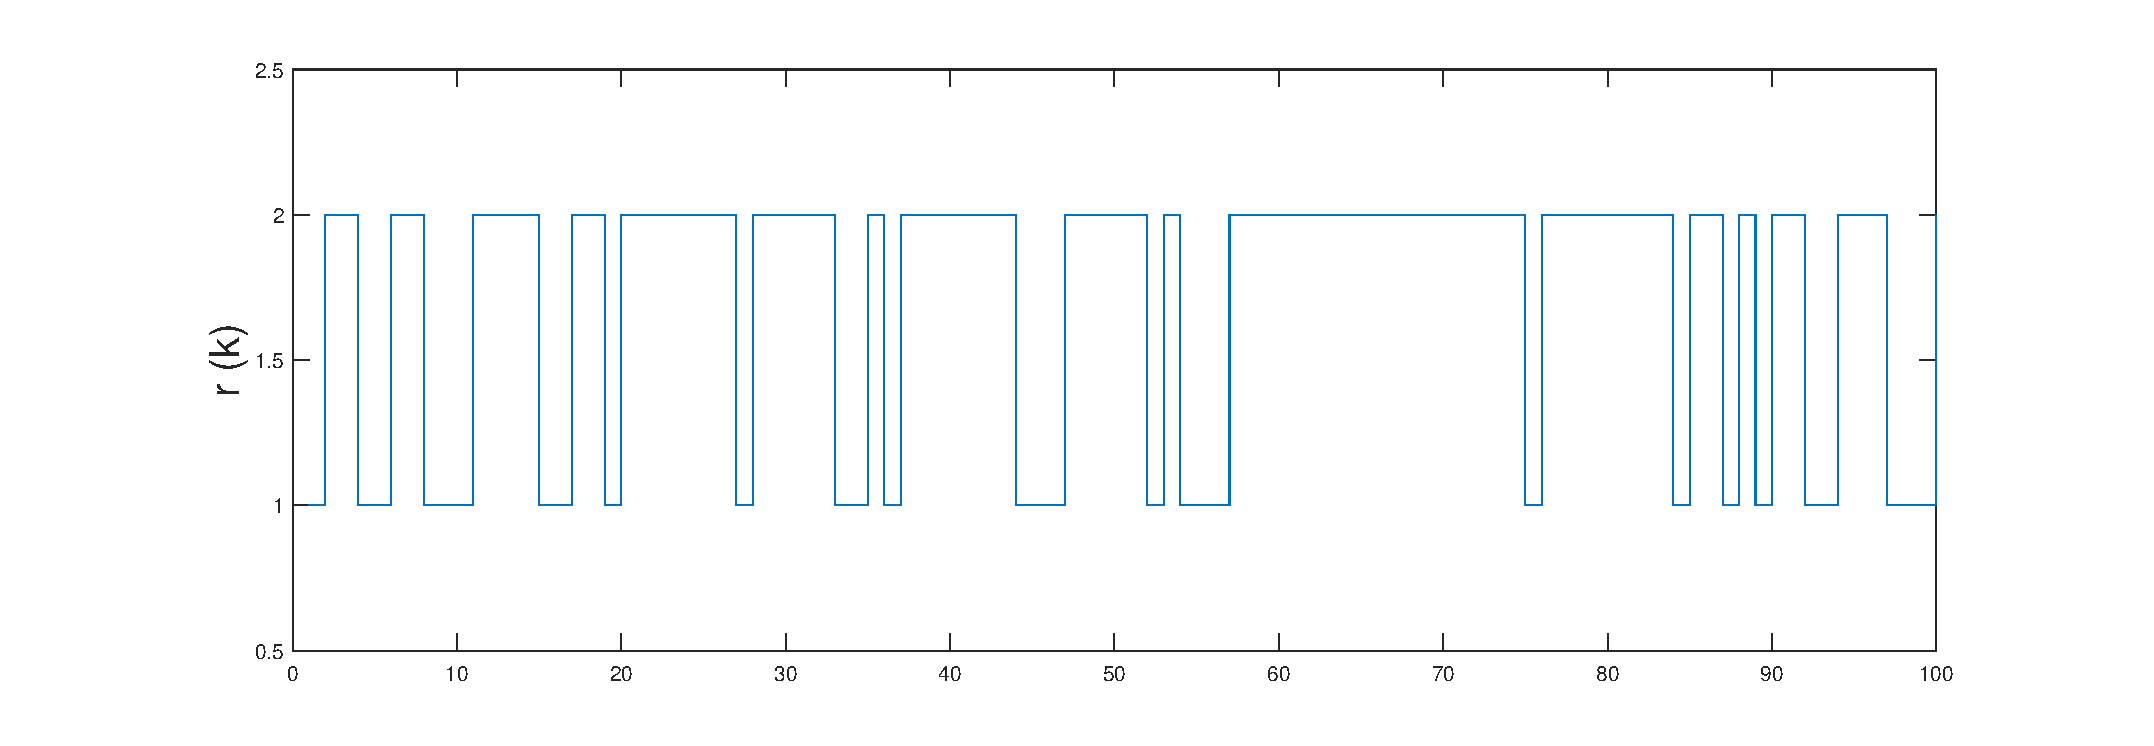
\includegraphics[scale=0.25]{./simulink/mode_p.eps}\\ 
 	\centering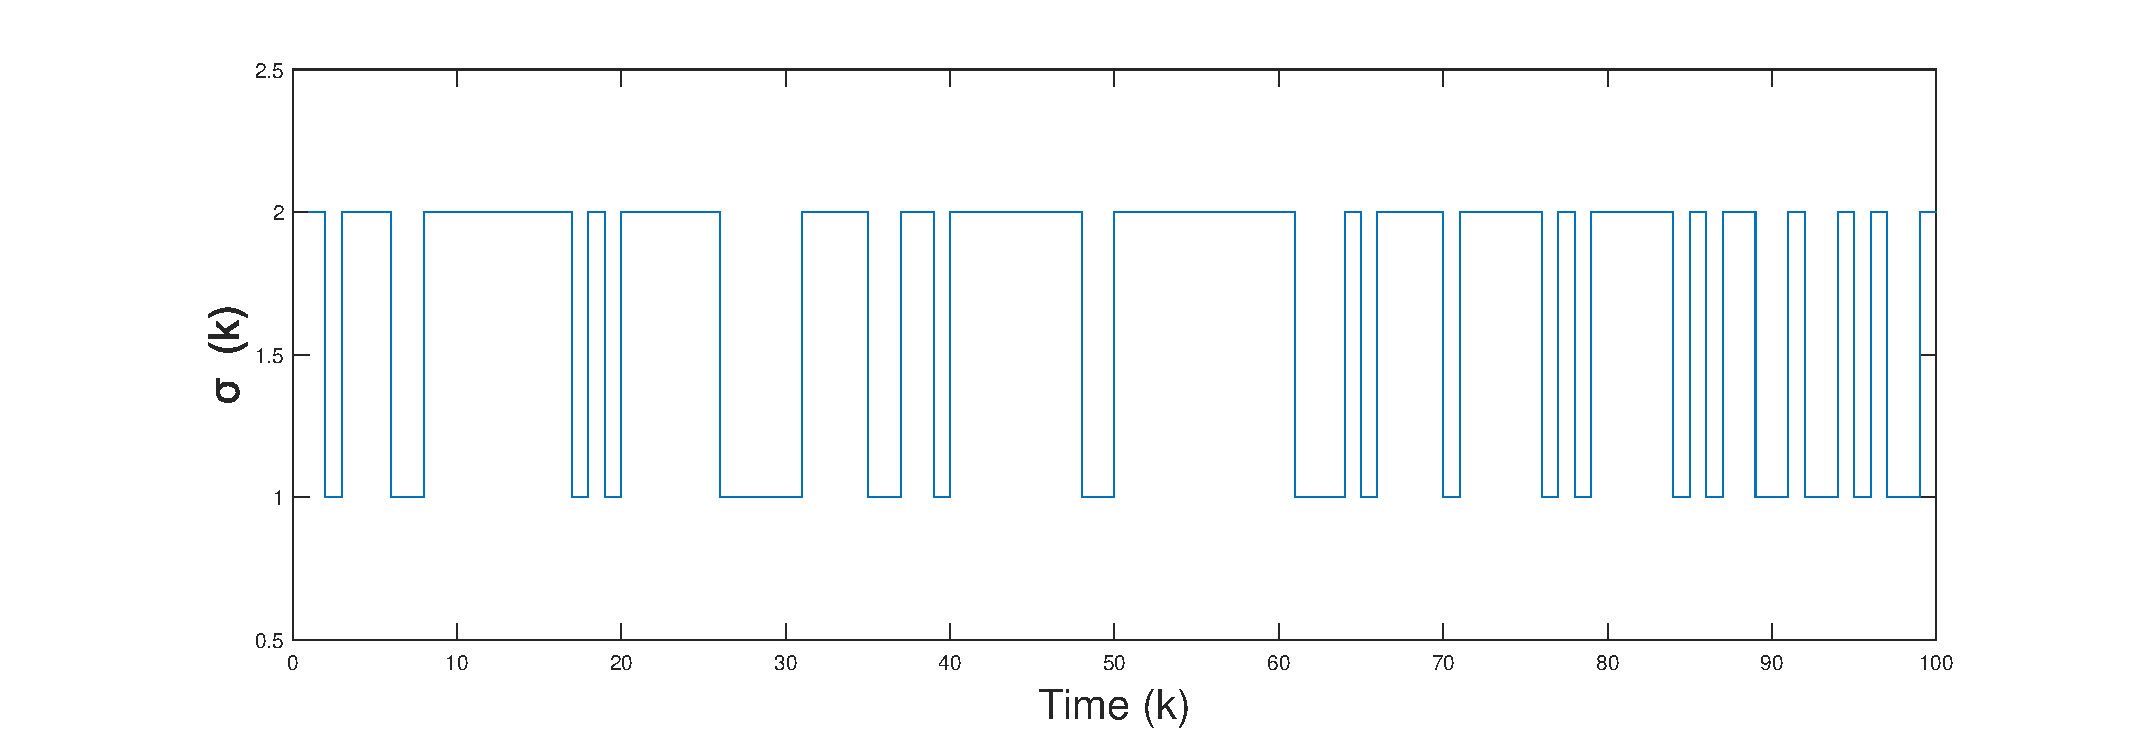
\includegraphics[scale=0.25]{./simulink/mode_k.eps}\\ 
	\caption{Modes of system and controller}
	\label{fig.1}
\end{figure}

\begin{figure}[!htb]
	\centering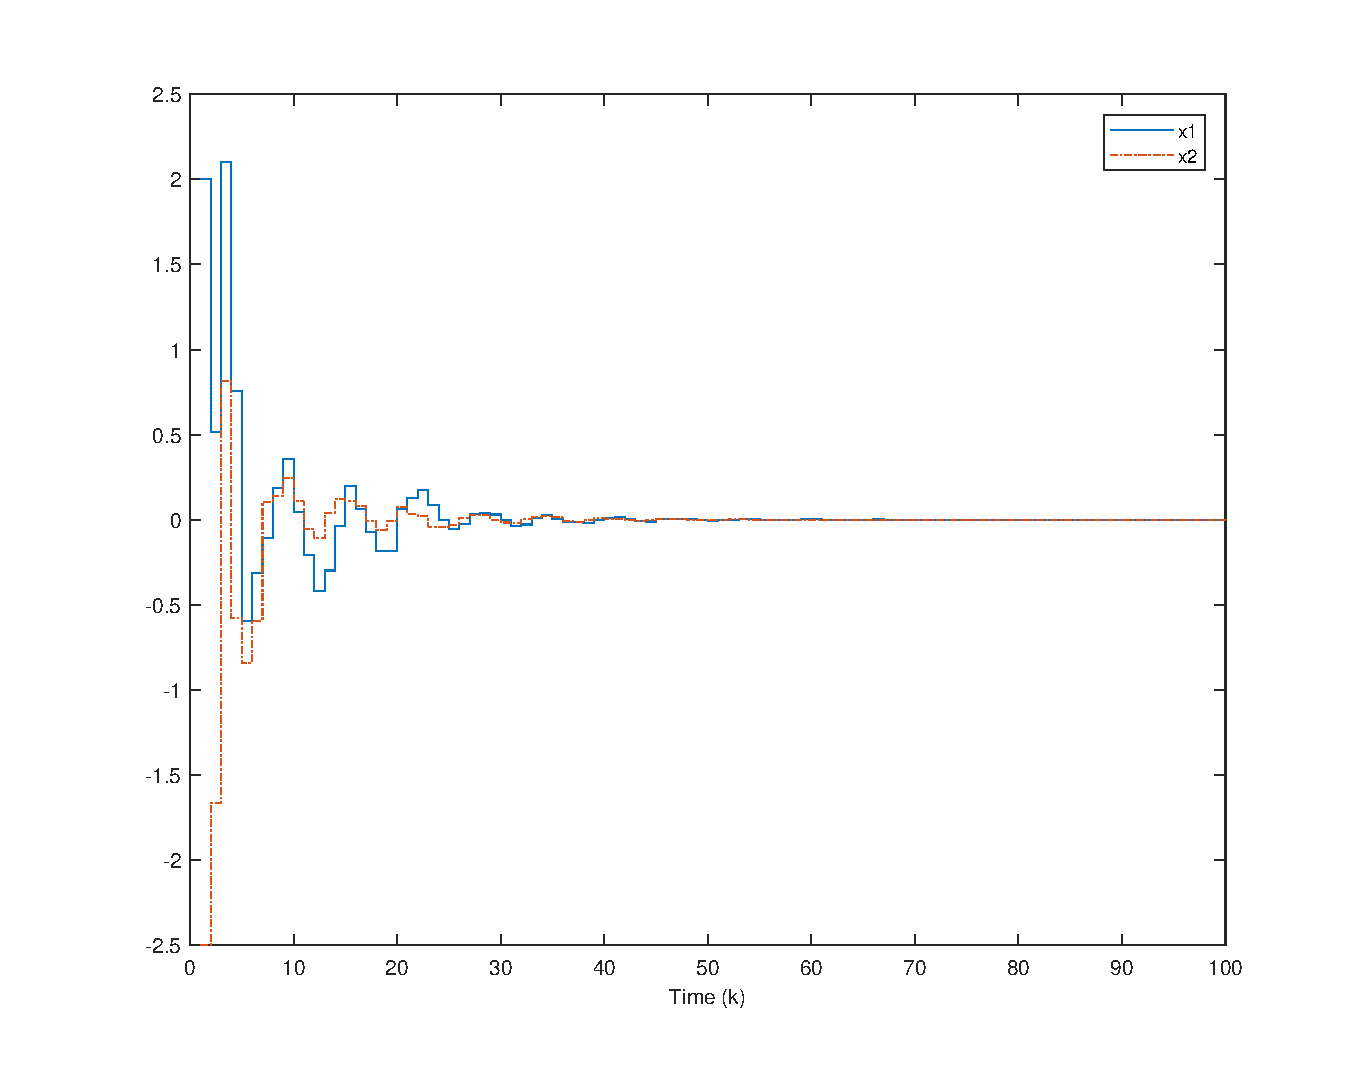
\includegraphics[scale=0.4]{./simulink/state_new.eps}\\
	\caption{System state}
	\label{fig.2}
\end{figure}
\begin{figure}[!htb]
	\centering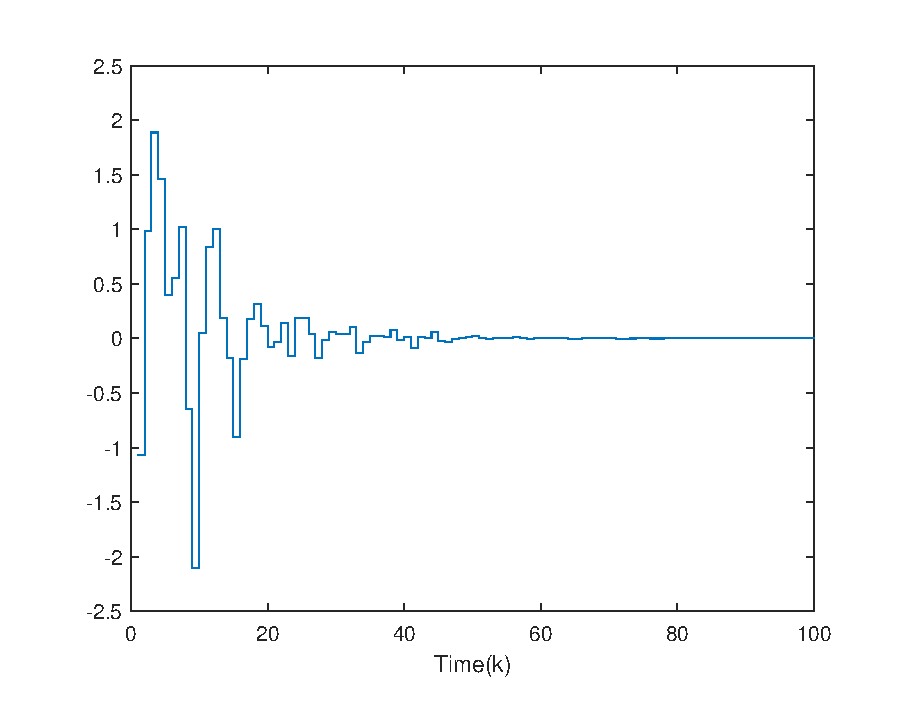
\includegraphics[scale=0.59]{./simulink/u_k3.eps}\\
	\caption{System input}
	\label{fig.3}
\end{figure}
Fig.1 gives a possible time sequences of the mode of system and asynchronous controller. We select the initial state $x_{0}=\begin{bmatrix}
	2&-2.5
\end{bmatrix}^{'}$, and the external disturbance is assumed to be $w_{k} = sin(k)*0.9^{k}$. Then we can get state response of system, which is depicted in Fig.2.



\section{Conclusions}
The stochastic stabilization and $l_{2}$-gain  minimization problems for a class of discrete-time nonlinear Markov systems with asynchronous controller have been discussed in this paper. 

% conference papers do not normally have an appendix

% use section* for acknowledgment
\section*{Acknowledgment}


The authors would like to thank...


\begin{thebibliography}{1}
	\bibitem{zyf}
	Zhu Y, Zhang L, Zheng W X. Distributed ${\mathcal{H_{\infty}}}$ Filtering for a Class of Discrete-Time Markov Jump Lur’e Systems With Redundant Channels[J]. IEEE Transactions on Industrial Electronics, 2016, 63(3):1876-1885.
	
	\bibitem{mode_independent_T}
	Todorov M G, Fragoso M D. New methods for mode-independent robust control of Markov jump linear systems[J]. Systems \& Control Letters, 2016, 90:38-44.
	\bibitem{mode_independent_wuhuaining}
	Wu, H. N., \& Cai, K. Y. (2006). Mode-independent robust stabilization for uncertain markovian jump nonlinear systems via fuzzy control. IEEE Transactions on Systems Man \& Cybernetics Part B Cybernetics A Publication of the IEEE Systems Man \& Cybernetics Society, 36(3), 509-19.
	
	\bibitem{passive_wu}
	Wu, Zheng Guang, et al. "Passivity-Based Asynchronous Control for Markov Jump Systems." IEEE Transactions on Automatic Control 62.4(2017):2020-2025.
	
	\bibitem{l2_filter_wu}
	Z.-G. Wu, P. Shi, H. Su, and J. Chu, “Asynchronous $l_{2}$-$l_{\infty}$ filtering for discrete-time stochastic Markov jump systems with randomly occurred sensor nonlinearities,” Automatica, vol. 50, no. 1, pp. 180–186, 2014. 
	
	\bibitem{dispassive-control-wu}
	Z.-G. Wu, S. Dong, H. Su, and C. Li, “Asynchronous dissipative control for fuzzy Markov jump systems,” IEEE Trans. Cybern., to be published, doi: 10.1109/TCYB.2017.2739754.
	
	\bibitem{filter_shenying}
	Shen Y, Wu Z G, Shi P, et al. Asynchronous Filtering for Markov Jump Neural Networks With Quantized Outputs[J]. IEEE Transactions on Systems Man \& Cybernetics Systems, 2018, PP(99):1-11.
	
	\bibitem{continus_filter_dongshanling}
	Dong, Shanling, et al. "Hidden-Markov-Model-Based Asynchronous Filter Design of Nonlinear Markov Jump Systems in Continuous-Time Domain." IEEE Transact  ions on Cybernetics PP.99:1-11.
	
	\bibitem{filter_zhangmeng}
	Zhang M, Shi P, Liu Z, et al. Fuzzy Model-based Asynchronous H $\infty$ Filter Design of Discrete-Time Markov Jump Systems[J]. Journal of the Franklin Institute, 2017, 354(18).
	
	\bibitem{unknown_asynchronous_control}
	Song, Jun, et al. "Finite-time $l_2$-$l_\infty$ control of Markovian jump linear systems with partly accessible hidden information via asynchronous output feedback." Control Conference IEEE, 2018:2447-2452.
	
	\bibitem{khnlil}
	Khalil, H. K. (2002). Nonlinear systems (3rd ed.). Prentice Hall
	
	\bibitem{state_output_control_EB}
	Castelan E B, Moreno U F, Pieri E R D. Absolute stabilization of discrete-time systems with a sector bounded nonlinearity under control saturations[C]// IEEE International Symposium on Circuits and Systems, 2006. ISCAS 2006. Proceedings. IEEE, 2006:4 pp.
	
	\bibitem{state_output_control_EB_continues}
	Castelan E B, Tarbouriech S, Queinnec I. Control design for a class of nonlinear continuous-time systems ☆[J]. Automatica, 2008, 44(8):2034-2039.
	
	\bibitem{song_control}
	Song G, Zhang Y, Xu S. Stability and l 2 -gain analysis for a class of discrete-time non-linear Markovian jump systems with actuator saturation and incomplete knowledge of transition probabilities[J]. Iet Control Theory \& Applications, 2012, 6(17):2716-2723.
	
	\bibitem{gonzaga}
	Gonzaga, Carlos A. C., M. Jungers, and J. Daafouz. "Stability analysis of discrete-time Lur’e systems ☆." Automatica 48.9(2012):2277-2283.
	
	\bibitem{costaolv_control_1}
	Gonzaga C A C, Jungers M, Daafouz J. Stability analysis of discrete-time Lur’e systems ☆[J]. Automatica, 2012, 48(9):2277-2283.
	
	\bibitem{costaolv_control}
	Gonzaga C A C, Costa O L V. Stochastic stabilization and induced ℓ 2 -gain for discrete-time Markov jump Lur'e systems with control saturation[M]. Pergamon Press, Inc. 2014.
	
\end{thebibliography}




% that's all folks
\end{document}





